\section{目的}
依 Lab 12（PDF 52--54 頁）比較尺寸對五級延遲元件的影響，並尋找固定五級、2 pF 負載下的較佳級間放大率。

\section{Spec 對照}
\begin{longtable}{p{0.31\linewidth}p{0.29\linewidth}p{0.31\linewidth}}
\toprule
講義要求（PDF頁） & 實作 & 驗證與界線 \\\midrule
步驟 1：表 12.1 四種尺寸（52、54） & 01\_delay\_elements & 四個五級鏈並列 \\
步驟 2：改變 taper n（53--54） & 02\_taper\_buffer & 五級，n=2/3/4/5，$C_L=2$ pF \\
\bottomrule
\end{longtable}


\section{電路與設計推導}
第一部分嚴格採表 12.1 的四組 $W_p,W_n,L$。其中 case 2 表列 $W_p=1.2\,\mu$m，正文卻說是 case 1 的一半（應為 1.8）；本文依表實作並保留此歧義。原始程式改變了尺寸及比例，已恢復講義表格。第二部分第 k 級的寬度為第一級乘 $n^{k-1}$，固定 $L=0.25\,\mu$m、第一級 $W_n/W_p=0.6/1.8\,\mu$m；末級接講義要求 2 pF，修正原始程式的 1 pF。

近似延遲 $t\sim RC$：加寬可減少通道電阻，卻增加下一級與自身寄生負載，因此總延遲不必單調減少。

\section{模擬設定}
本次為使用另行提供模型的教學改寫，電源為 1.0 V、溫度為 $25\,^{\circ}\mathrm C$。保留講義指定的拓樸、負載及比較尺寸；原講義的 2.5 V 製程結果不是本次模型的驗收數值。1 V 僅是模擬條件，不能視為模型的安全額定。所有 MOS 的 Bulk 明確接至相應電源軌。

HSPICE S-2021.09 使用 RUNLVL=6；保存波形、列印資料及原生量測。圖表由本次數據重繪；CSV 保存於各 Lab 的 results。完成模擬表示求解成功，並不代表製程可靠度已驗證。加密模型仍有被抑制的警告；既有診斷未取得可判讀的進一步內容，因此不宣稱警告無害或全部模型限制已滿足。

延遲鏈輸入邊緣 0.1 ns、週期 5 ns、模擬 15 ns；taper 使用相同邊緣，初始延遲 2 ns、脈寬 20 ns、週期 45 ns、模擬 90 ns，確保大負載充分轉換。所有延遲均量輸入 50\% 至第五級相反方向 50\%，分列 $t_{pHL},t_{pLH}$。

\section{結果與規格檢查}
全部五個參數案例正常。尺寸單位 $\mu$m，延遲單位 ns。
\begin{center}\small
\begin{tabular}{llllll}
\toprule
Case & $W_p$ & $W_n$ & $L$ & $t_{pHL}$ & $t_{pLH}$ \\
\midrule
1 & 3.6 & 1.2 & 0.25 & 0.3634 & 0.3786 \\
2 & 1.2 & 1.2 & 0.25 & 0.3515 & 0.3926 \\
3 & 3.6 & 1.2 & 0.5 & 1.2781 & 1.3400 \\
4 & 1.8 & 1.2 & 0.5 & 1.2200 & 1.3434 \\
\bottomrule
\end{tabular}
\end{center}

\begin{figure}[htbp]
\centering
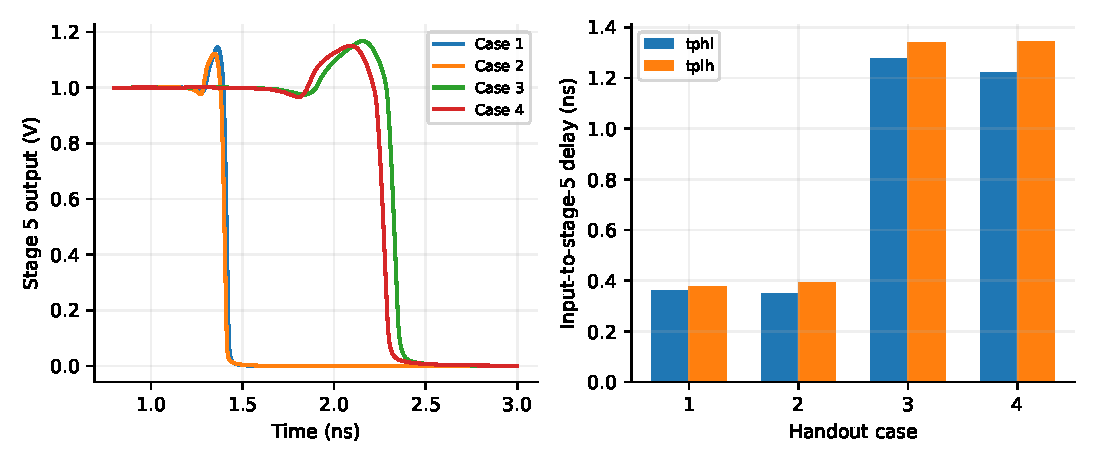
\includegraphics[width=\linewidth]{figures/delay_elements.pdf}
\caption{四種延遲元件尺寸的結果；由本次 HSPICE 數據重繪。}
\end{figure}
\begin{center}\small
\begin{tabular}{llll}
\toprule
n & $t_{pHL}$ (ns) & $t_{pLH}$ (ns) & Mean (ns) \\
\midrule
2 & 0.9314 & 1.1852 & 1.0583 \\
3 & 0.8779 & 0.9877 & 0.9328 \\
4 & 0.9924 & 1.3381 & 1.1652 \\
5 & 1.5245 & 2.2524 & 1.8884 \\
\bottomrule
\end{tabular}
\end{center}

\begin{figure}[htbp]
\centering
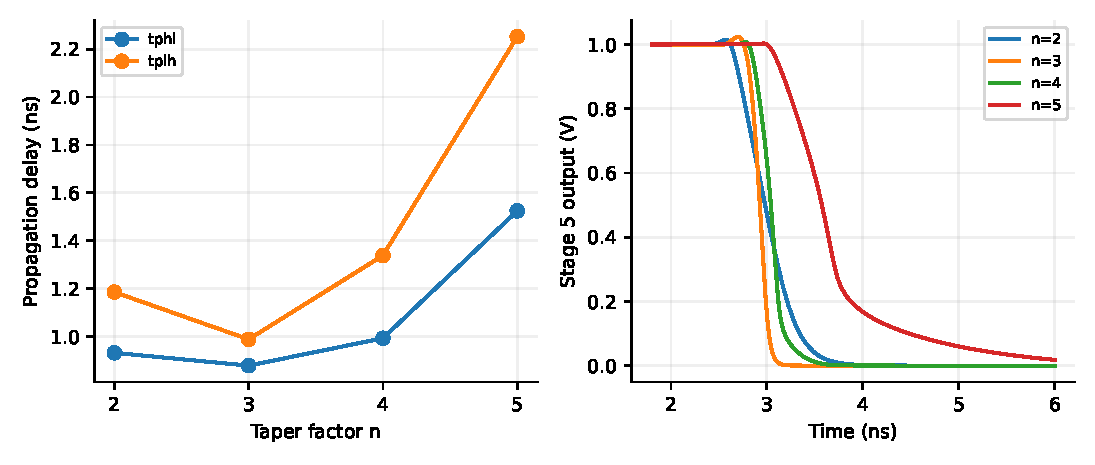
\includegraphics[width=\linewidth]{figures/taper_buffer.pdf}
\caption{固定五級與 2 pF 的 taper 比較；由本次 HSPICE 數據重繪。}
\end{figure}


\section{討論}
四組尺寸顯示加長通道明顯增加延遲，但降低 PMOS 寬度對上升／下降延遲的影響不同。此模型的表 case 1/2 平均延遲幾乎相同，因此不能沿用講義單一 delay 的排序作普遍結論。在測試的 n=2--5 中，n=3 的平均延遲約 0.933 ns 最小，與講義最佳 n 的趨勢一致，但數值不是其 0.449 ns。未搜尋其他級數、非等比尺寸或不同負載，故不稱全域最佳化。

\section{結論}
兩個步驟完整覆蓋；尺寸歧義採表格、2 pF 負載與五級結構均明確。結論是本次條件下的有限參數比較。
